%% LyX 2.3.6.1 created this file.  For more info, see http://www.lyx.org/.
%% Do not edit unless you really know what you are doing.
\documentclass[11pt,a4paper,english]{desearticle_1col}
\usepackage{mathptmx}
\usepackage{helvet}
\usepackage{courier}
\renewcommand{\familydefault}{\rmdefault}
\usepackage[latin9]{inputenc}
\usepackage{fancyhdr}
\pagestyle{fancy}
\usepackage{float}
\usepackage{booktabs}
\usepackage{graphicx}

\makeatletter

%%%%%%%%%%%%%%%%%%%%%%%%%%%%%% LyX specific LaTeX commands.
\pdfpageheight\paperheight
\pdfpagewidth\paperwidth

%% Because html converters don't know tabularnewline
\providecommand{\tabularnewline}{\\}

%%%%%%%%%%%%%%%%%%%%%%%%%%%%%% User specified LaTeX commands.
\Author{Guhan Rajasekar(22410), Harivignesh(23409)}
\Afil{DESE, IISc}
\Journal{Digital System Design With FPGA}
\Month{Jan-Apr}
\Year{2024}

\makeatother

\usepackage{babel}
\begin{document}
\title{{\huge{}Trignometric Functions Generation Using CORDIC}}
\maketitle

\section{Introduction and Motivation}
\begin{itemize}
    \item This report is a summary on generation of various trigonometric functions using CORDIC (\textit{Coordinate Rotation Digital Computer})algorithm.
    \item Motivation behind using this algorithm is to demonstrate the feasibility of generating various mathematical functions in a hardware friendly manner. When we say hardware friendly, we mean, we mean avoiding usage of multiplier blocks of FPGA and generating the functions using shift and add operations. 
    \item There are other methods to generate trigonometric functions like \textit{Taylor's Series Expansion , Look Up Table Based Generation etc}. But these techniques are not hardware friendly and are very resource intensive. Hence this gives us clear motivations to use CORDIC to implement the said functionalities with economic usage of the available hardware resources. 

    \item In this project, we demonstrate the implementation of sin, cos, tan, tan inverse, tan hyperbolic and tan hyperbolic inverse functions with CORDIC.
\end{itemize}

\section{Back Ground Study}
\subsection{Generalized Equations Of CORDIC}
\begin{itemize}
    \item The generalized equations of CORDIC are given as : 
     \begin{equation}
         x^{(i+1)} = x^{(i)} - \mu d_{i}(2^{-i}y^{(i)})
     \end{equation}
    
     \begin{equation}
         y^{(i+1)} = y^{(i)} + d_{i}(2^{-i}x^{(i)})
     \end{equation}
     
     \begin{equation}
         z^{(i+1)} = z^{(i)} - d_{i}e^{i}
     \end{equation}

     \begin{equation}
         \textit{Circular Rotations}: \mu = 1 , e^{i} = tan^{-i}2^{-i}
     \end{equation}

     \begin{equation}
         \textit{Linear Rotations}: \mu = 0, e^{i} = 2^{-i} 
     \end{equation}

     \begin{equation}
         \textit{Hyperbolic Rotations}: \mu = -1 , e^{i} = tanh^{-i}2^{-i}
     \end{equation}       
\end{itemize}

\subsection{Modes Of CORDIC Algorithm}
\begin{itemize}
    \item CORDIC operates in any one of the following two modes: 
    \begin{itemize}
        \item \textit{Rotation Mode}:$d_{i}$ = signum($z^i$)

        \item \textit{Vectoring Mode}: $d_{i}$ = -signum($x^{i}y^{i}$)
    \end{itemize}
\end{itemize}

\subsection{Convergence of CORDIC}
\begin{itemize}
    \item For Sin and Cos function implementation, CORDIC algorithm works fine when the angle lies between $-90^o$ and $90^o$. For angles lying outside this range, we apply standard trignometric identities to get the desired result. 

    \item Elemental rotations using Hyperbolic CORDIC will not converge. Convergence is guaranteed if the following iterations are repeated : 4, 13, 40,.......k,(3k+1). We do not deal with the exact math behind this as it is beyond the scope of this project.
\end{itemize}

\newpage

\section{Implementation Of The Various Trigonometric Functions Using CORDIC}
\subsection{Sin and Cos Functions Generation using CORDIC}
\begin{itemize}
    \item Both sin and cos functions are implemented using \textit{Circular Rotations} in \textit{Rotation Mode}.

    \begin{figure}[H]
        \centering
        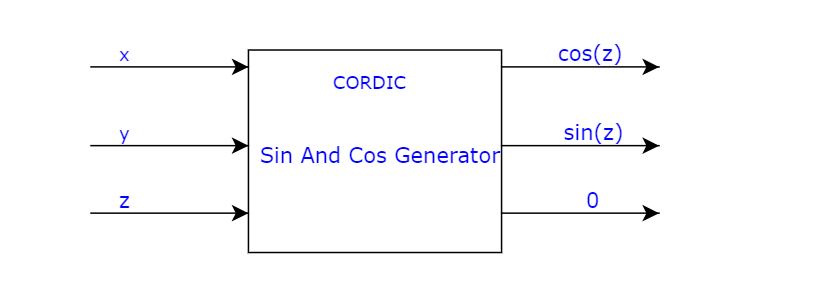
\includegraphics[width=0.8\textwidth, height = 5cm]{sin_cos_block.png}
        \caption{Block Diagram Of Sin and Cos generation}
        \label{fig:enter-label}
    \end{figure}

   \item x is initialized with value 0.6073, y with 0 and z holds the angle value for which we need to find sin and cos values. 10 iterations have been carried out in this project. After 10 iterations, x converges to cos(z) , y converges to sin(z) and z converges to 0. 

   \item To implement this, we use 10 iterations in a combinational always block [i.e, always@(*) ]. When the 10 iterations are over, the final result is updated in a separated register. This final updated happens in a clocked always block [i.e, always@(posedge clk) ]. 
\end{itemize}

    \subsubsection{Resource Utilization of Sin and Cos }
    \begin{figure}[H]
        \centering
        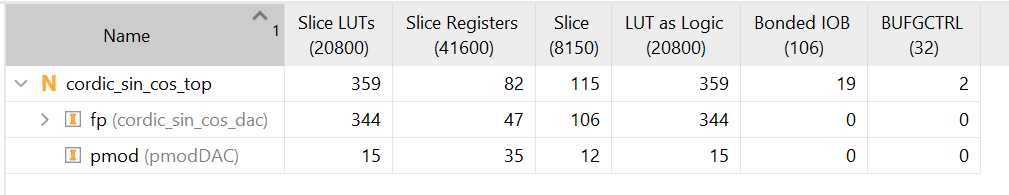
\includegraphics[width=0.8\textwidth]{resource_utilization_sin_cos.png}
        \caption{Resource Utilization of Sin And Cos Generator Block}
        \label{fig:enter-label}
    \end{figure}

    \subsubsection{Post Implementation Timing Results of Sin and Cos Generator Block}
    \begin{figure}[H]
        \centering
        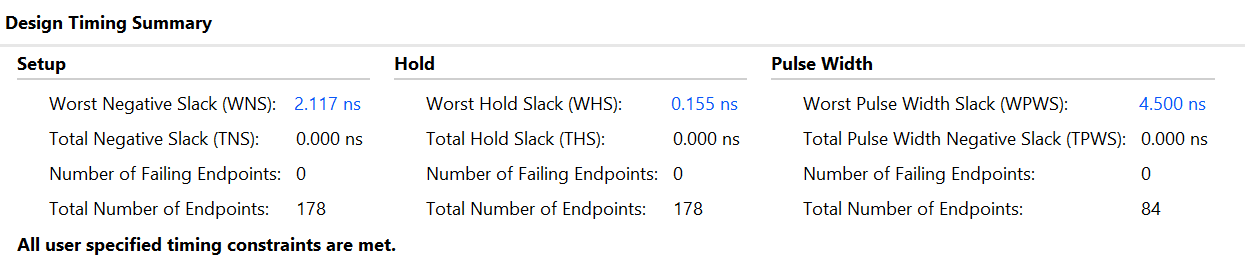
\includegraphics[width=0.8\textwidth]{sin_cos_timing_results.png}
        \caption{Post Implementation Timing Results of Sin And Cos Generator Block}
        \label{fig:enter-label}
    \end{figure}

    \begin{itemize}
        \item Although we get a positive slack of 2.117ns with the 100MHz, since we are using the PMOD DAC, max frequency of operation is limited to 30MHz
    \end{itemize}

  \subsubsection{Viewing Sin and Cosine Waveforms on the Oscilloscope using PMOD DA2 DAC}
     \begin{itemize}
         \item The sin and cos values generated were also viewed on the oscilloscope using PMOD DA2 DAC. The DAC can operate at a maximum frequency of 30MHz. So we generate the sin and cosine values at a rate that is much slower than 30MHz. 
         \item For this purpose, we use the original clock of 100MHz to generate a slower clock signal of 3.33MHz. Any value less than 30MHz would work.
         \item The user provides a 12 input using the slide switches present on the FPGA. As the slide switch input given by the user increases, the frequency of the waveform increases and as we move to higher frequencies, distortion also increases. This is because of the limits imposed by the conversion time of the DAC, which is at 10$\mu$s.
         \item While sending the values to the DAC, the sine and the cosine values that are generated also need to be up-shifted by a certain amount as the DAC can handle values only between 0 and 4095.
    
    \begin{figure}[H]
        \centering
        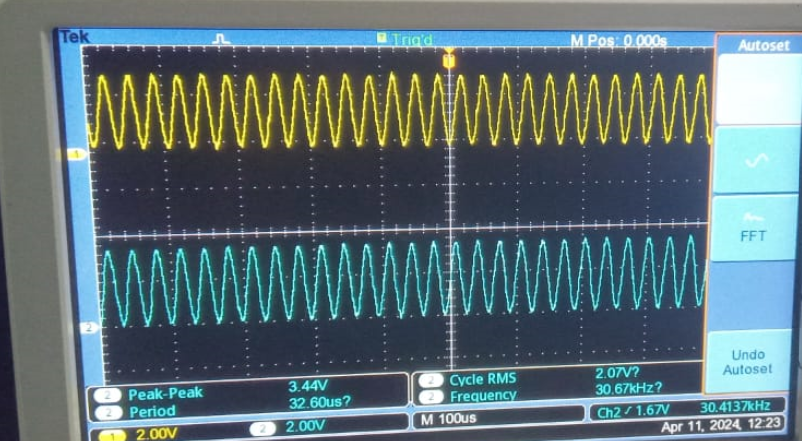
\includegraphics[width=12cm, height = 5cm]{sin_cos_scope_diagrams.png}
        \caption{Sin and Cos Waveforms observed on Oscilloscope}
        \label{fig:enter-label}
    \end{figure}     
\end{itemize}

\subsection{Tan Function Generation Using CORDIC}
\begin{itemize}
    \item While it is not possible to directly generate tan waveforms, we perform division through CORDIC. We take the results of sin and cos that were generated through CORDIC and pass them to the CORDIC divider block to get tan waveform. CORDIC divider works in \textit{Linear Rotations} in \textit{Vectoring Mode}.  In this method, the \textit{z} of the divider block converges to tan of the given angle. \textit{y} of the divider block converges to 0 and the value that \textit{x} of the divider block converges to is of no consequence to us. 

    \begin{figure}[H]
        \centering
        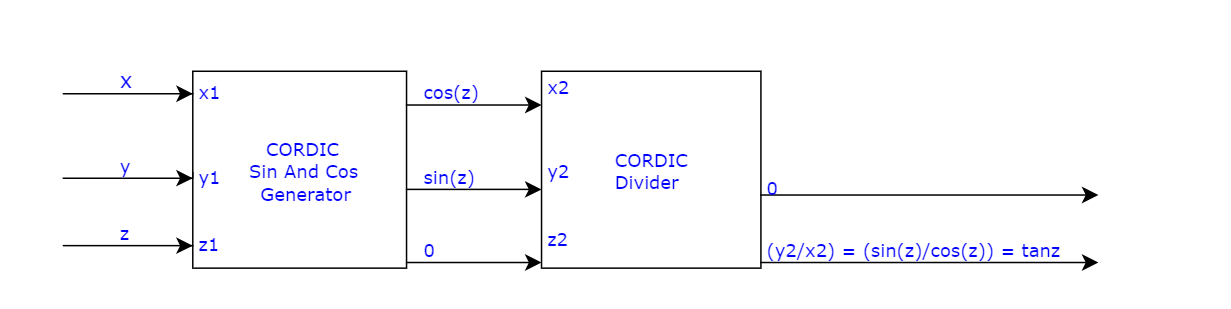
\includegraphics[width=18cm, height = 4.0cm]{tan_block_diagram_updated.png}
        \caption{Block Diagram of Tan Generation}
        \label{fig:enter-label}
    \end{figure}
\end{itemize}
\subsubsection{Limitations Of CORDIC Division}
\begin{itemize}
    \item The iterative expression for \textit{z} component of the CORDIC divider is given as :
    \begin{equation}
        z^{(i+1)} = z^{(i)} - d_i2^{(-i)}
    \end{equation}
    \item Here at each iteration $d_i$ can be either +1 or -1. The max value that z can take in the first iteration is 1. The max value in the second iteration is 1 + $\frac{1}{2}$. The max value in the third step is 1 + $\frac{1}{2}$ + $\frac{1}{4}$. This is a geometric progression that converges to 2 after infinite iterations. Hence the max positive value that CORDIC division gives is +2 and the max negative value that CORDIC division gives is -2. Because of this, the tan waveform that is obtained through CORDIC also lies in the range of [-2,2].
\end{itemize}

\subsubsection{Resource Utilization Of Tan Generator Block}
    \begin{figure}[H]
        \centering
        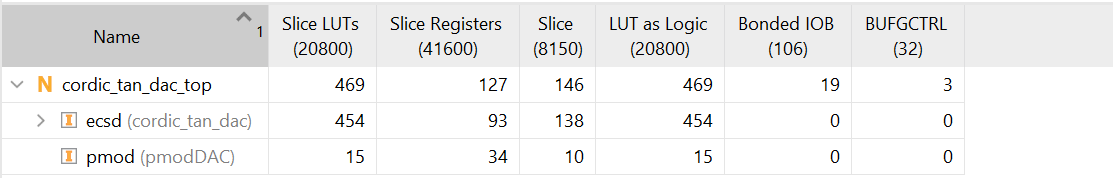
\includegraphics[width=0.8\textwidth]{tan_resource_utilization.png}
        \caption{Resource Utilization Of Tan Generator Block}
        \label{fig:enter-label}
    \end{figure}    

\subsubsection{Post Implementation Timing Results of Tan Generator Block}
    \begin{figure}[H]
        \centering
        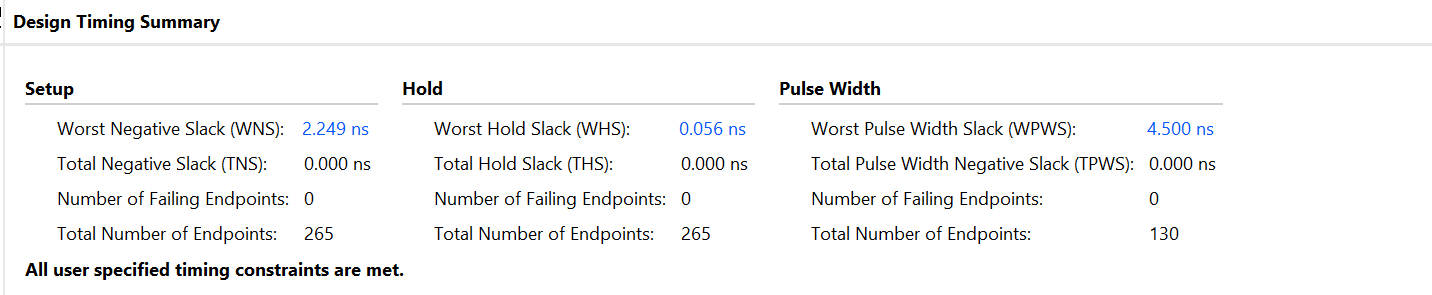
\includegraphics[width=0.8\textwidth]{tan_timing_results.png}
        \caption{Post Implementation Timing Results Of Tan Generator Block}
        \label{fig:enter-label}
    \end{figure} 
    
    \begin{itemize}
        \item Max operating frequency of the Tan Generator Block is 30MHz. This limitation is imposed by the PMOD DA2 DAC that is used to display the tan waveform on the Oscilloscope. 
    \end{itemize}

\subsubsection{ Expected Tan Waveform Vs Post Implementation Simulation Tan Waveform }
    \begin{figure}[H]
        \centering
        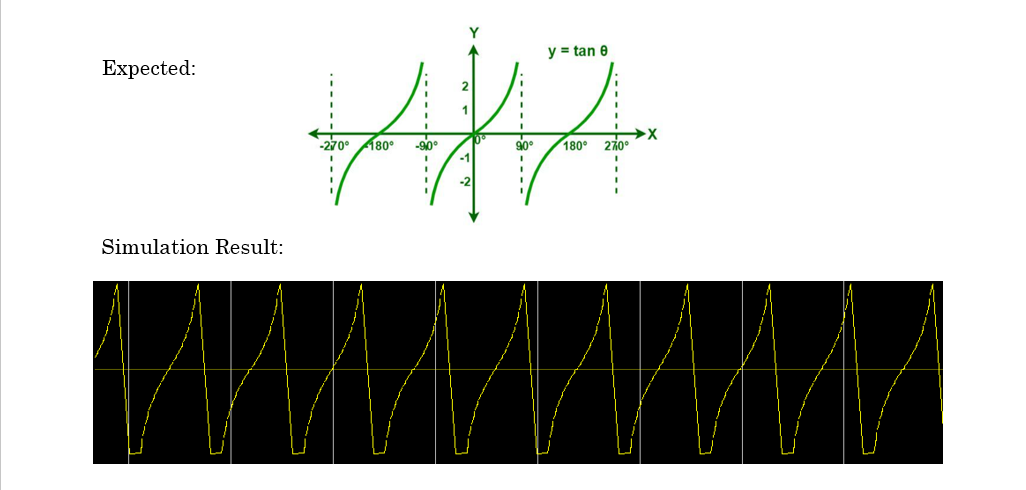
\includegraphics[width=18cm, height = 5.0cm]{tan_expected_vs_simulation.png}
        \caption{Comparison of Expected Vs Post Implementation Simulation Waveform of Tan}
        \label{fig:enter-label}
    \end{figure}     

\subsubsection{Viewing Tan Waveforms On Oscilloscope Using PMOD DA2 DAC}
    \begin{figure}[H]
        \centering
        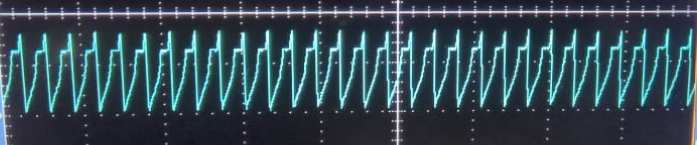
\includegraphics[width=18cm, height = 3.0cm]{tan_waveform_scope.png}
        \caption{Tan Waveform On The Oscilloscope}
        \label{fig:enter-label}
    \end{figure} 
    \begin{itemize}
        \item To send the Tan values to the DAC, an offset of 1024 is added to all the values generated in the program to get it within the range that can be handled by the DAC. When this is done, a small portion on the top half of the tan waveform is being clipped and becomes flat. This part needs further investigation. 
    \end{itemize}

\subsection{Tanh Inverse Function Generation Using CORDIC}
\bibliography{report}
    \begin{figure}[H]
        \centering
        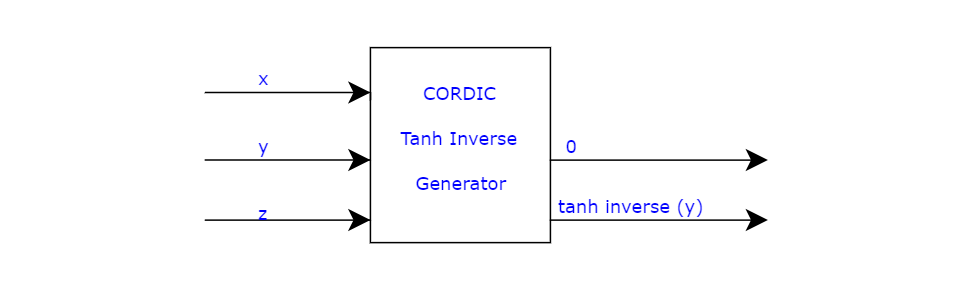
\includegraphics[width=0.75\textwidth, height = 4cm ]{tanh_inverse_block_diagram.png}
        \caption{Block Diagram Of Tanh Inverse Generator}
        \label{fig:enter-label}
    \end{figure} 
  \begin{itemize}
      \item To get $tanh^{-1}(y)$, we initialize x with 1 and z with 0. After 10 iterations ( Number of iterations is designers' choice), y converges to 0, z converges to $tanh^{-1}(y)$ and the value that x converges is of no consequence to us. 
  \end{itemize}

\subsubsection{Resource Utilization Of Tanh Inverse Generator}
    \begin{figure}[H]
        \centering
        
\includegraphics[width=0.8\textwidth]{tanh_inverse_resource_utilization.png}
        \caption{Resource Utilization of tanh inverse generator}
        \label{fig:enter-label}
    \end{figure} 

\subsubsection{Post Implementation Timing Results Of Tanh Generator}
    \begin{figure}[H]
        \centering
        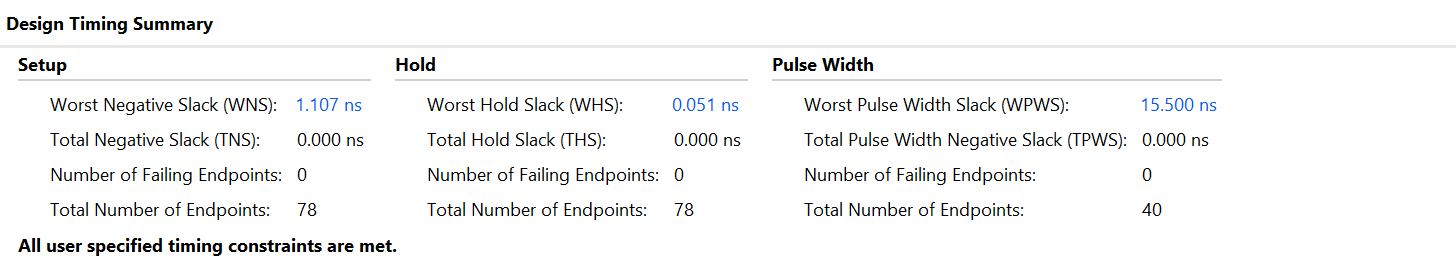
\includegraphics[width=0.8\textwidth]{tanh_inverse_timing.png}
        \caption{Post Implementation Timing Results Of Tanh Inverse Generator}
        \label{fig:enter-label}
    \end{figure} 
\begin{itemize}
    \item The tanh inverse block was operated with clock period of 32ns. Hence the maximum operating frequency is given by:
    \begin{equation}
        f_{max} = \frac{1}{32n - 1.107n} = \frac{1}{30.893} = 32.369MHz.
    \end{equation}
\end{itemize}
\subsubsection{Limitations Of Tanh Inverse Generation Using CORDIC}
\begin{itemize}
    \item $tanh^{-1}(y)$ is not a bounded function. It tends to +$\infty$ as y tends to 1 and tends to -$\infty$ as y tends to -1.
    \item Hence $tanh^{-1}(y)$ cannot be accurately captured by CORDIC for all possible values of y. Beyond $|y|$ > 1, it gets difficult to capture the values of $tanh^{-1}(y)$  accurately due to fixed number of iterations used in CORDIC and also due to limitations imposed by fixed point representation.
    \item However, CORDIC algorithm gives values of $tanh^{-1}(y)$ with decent accuracy when y lies in the range of [-1,1]. 
\end{itemize}

\subsubsection{Expected Vs Post Implementation Waveforms of Tanh Inverse}
    \begin{figure}[H]
        \centering
        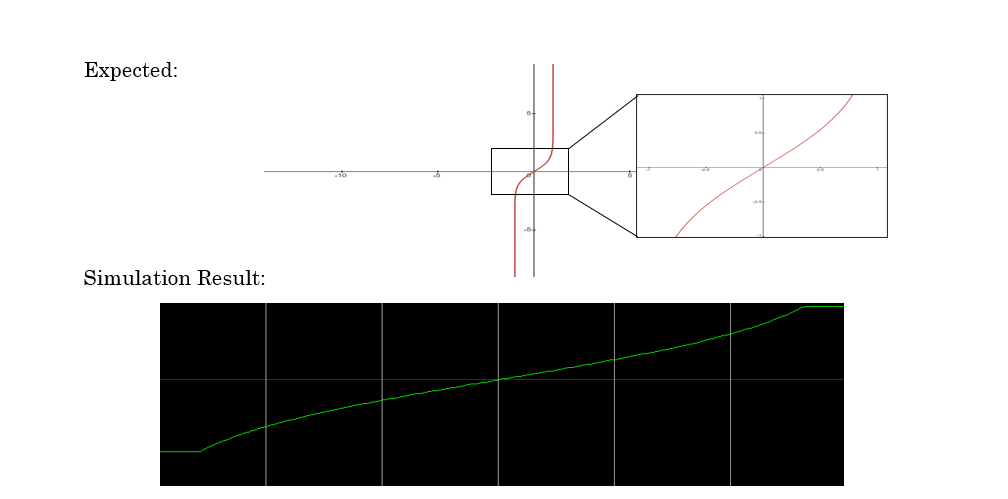
\includegraphics[width=0.8\textwidth , height = 6.5cm ]{tanh_inverse_comparision_diagram.png}
        \caption{Expected Waveform Vs Post Implementation Waveform of $tanh^{-1}(y)$}
        \label{fig:enter-label}
    \end{figure} 

\subsection{Tan Inverse Function Generation Using CORDIC}
    \begin{figure}[H]
        \centering
        
\includegraphics[width=18cm , height = 4cm ]{tan_inverse_block_diagram.png}
        \caption{Block Diagram of $tan^{-1}(y)$ Generator}
        \label{fig:enter-label}
    \end{figure} 
    \begin{itemize}
        \item $tan^{-1}(y)$ is obtained through \textit{Circular Rotations} in \textit{Vectoring Mode} of CORDIC.y value converges to 0 and the z value converges to $tan^{-1}(y)$. For this, x must be initialized to 1 and z must be initialized to 0.
    \end{itemize}

\subsubsection{Resource Utilization Of Tan Inverse Generator Block}
    \begin{figure}[H]
        \centering
        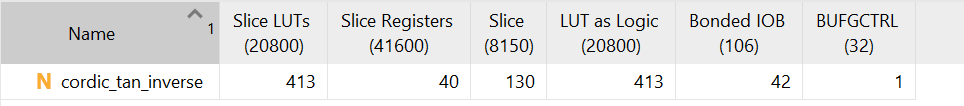
\includegraphics[width=0.8\textwidth]{tan_inverse_resource_utilzation.png}
        \caption{Resource Utilization of $tan^{-1}(y)$ Generator}
        \label{fig:enter-label}
    \end{figure} 

\subsubsection{Post Implementation Timing Results Of Tan Inverse Generator}
    \begin{figure}[H]
        \centering
        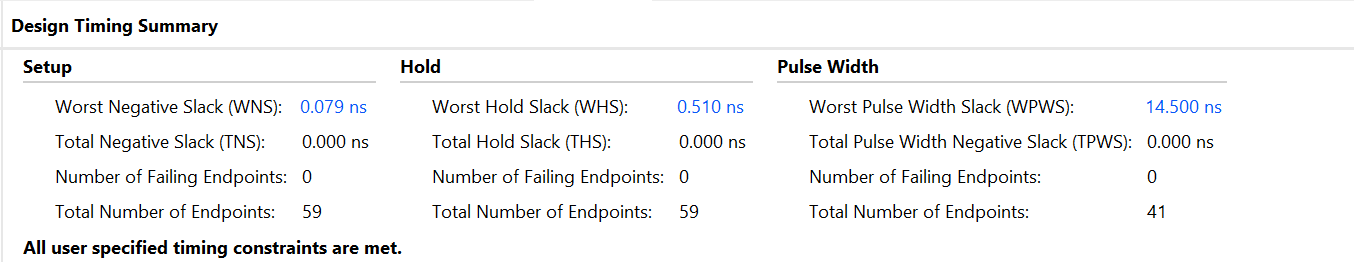
\includegraphics[width=0.8\textwidth , height = 2.0cm]{tan_inverse_timing_updated.png}
        \caption{Post Implementation of $tan^{-1}(y)$ Generator}
        \label{fig:enter-label}
    \end{figure} 
    \begin{itemize}
        \item The max operating frequency of $tan^{-1}(y)$ generator is:
        \begin{equation}
            f_{max} = 1/(30n - 0.079n) = 33.421\ MHz
        \end{equation}
    \end{itemize}

\subsubsection{Expected Vs Post Implementation Waveforms of Tan Inverse}
    \begin{figure}[H]
        \centering
        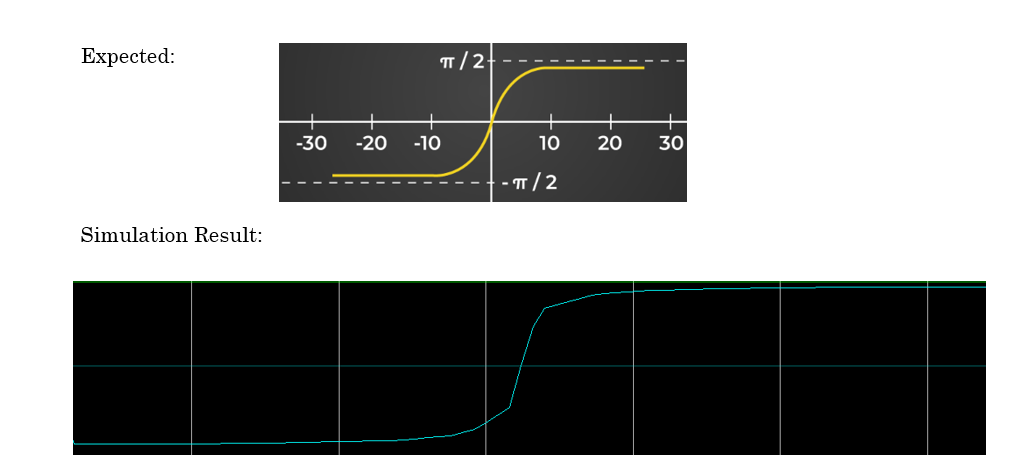
\includegraphics[width=0.8\textwidth , height = 6.0cm]{tan_inverse_comparision.png}
        \caption{Expected Vs Post Implementation Simulation Waveforms Of Tan Inverse Function}
        \label{fig:enter-label}
    \end{figure} 
    \begin{itemize}
        \item $tan^{-1}(y)$ function is generation very accurately by CORDIC directly through \textit{Circular Rotations} in \textit{Vectoring Mode} as it is a bounded function.
    \end{itemize}

\subsection{Tanh Function Generation Using CORDIC}
\begin{itemize}
    \item While it is not possible to generate tanh(z) function directly through CORDIC, we generate sinh(z) and cosh(z) directly through CORDIC and then pass the results through CORDIC Divider block to get tanh(z) function. 
    \begin{figure}[H]
        \centering
        
\includegraphics[width=0.8\textwidth]{tanh_block_diagram.png}
        \caption{Block Diagram Of Tanh Generator}
        \label{fig:enter-label}
    \end{figure}
    \item While generating sinh(z) and cosh(z), x is initialized to 1.2075, y is initialized to 0. z holds the angle value in radians initially. At the end of the fixed number of iterations, x converges to cosh(z) , y converges to sinh(z) and the z component converges to 0.
\end{itemize}

\subsubsection{Limitations Of Sinh And Cosh Function Generation Using CORDIC}
\begin{itemize}
    \item As was the case with $tanh^{-1}(y)$ generation, it is not possible to compute sinh(z) and cosh(z) for all values of z accurately using CORDIC. This is due to the fact that sinh(z) and cosh(z) are unbounded functions. When we deal with unbounded functions, accuracy is limited by the fixed number of iterations the algorithm employs and also by the fixed point representation used by the algorithm.

    \item Through simulation results, it was observed that sinh(z) and cosh(z) were obtained with good accuracy when z was within the range [-1,1]. 
    \item This is not a big problem as our main focus is on generating tanh(z). Because tanh(z) is 
    \textit{approximately} 1 for z greater than 1. So we use the values of the sinh(z) and cosh(z) from the first CORDIC stage and pass it on to the divider block to get tanh(z) values with good accuracy for z in the range of [-1,1]. Beyond [-1,1] , sinh(z) and cosh(z) values from the first CORDIC stage saturate to a fixed value. When these saturated values are passed to the CORDIC Divider block, we get the result to be 1 (approximately). So we get a reasonably good approximation of the tanh(z) 
    waveform.
\end{itemize}
\subsubsection{Resource Utilization Of Tanh Function Generation}
    \begin{figure}[H]
        \centering
        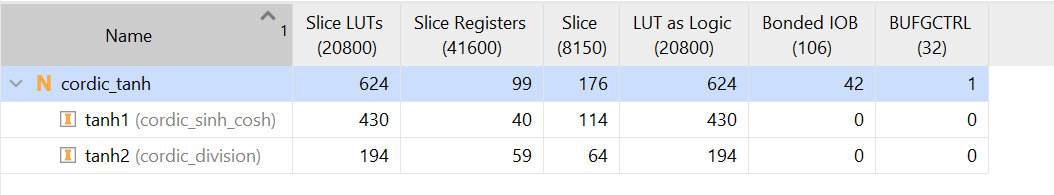
\includegraphics[width=0.8\textwidth]{tanh_resource_utilization.png}
        \caption{Resource Utilization Of Tanh Generator}
        \label{fig:enter-label}
    \end{figure}

\subsubsection{Post Implementation Timing Results Of Tanh Generator}
    \begin{figure}[H]
        \centering
        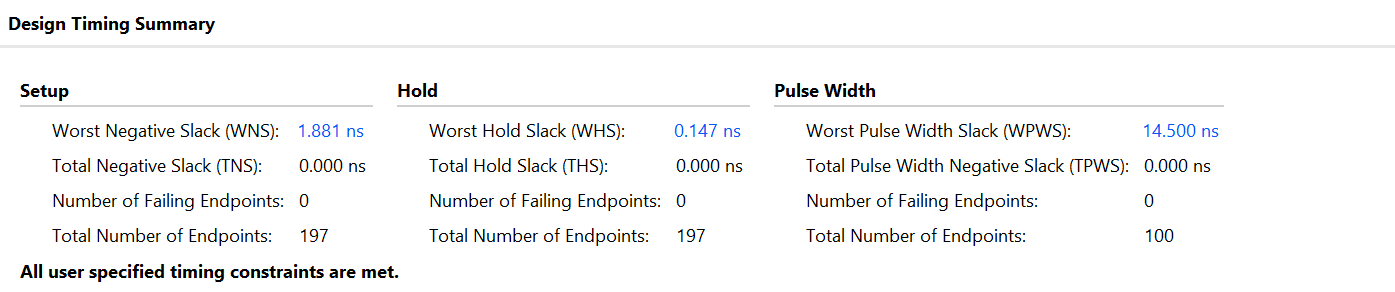
\includegraphics[width=0.8\textwidth]{tanh_timing_results.png}
        \caption{Post Implementation Timing Results Of Tanh Generator}
        \label{fig:enter-label}
    \end{figure}

\subsubsection{Expected Vs Post Implementation Simulation Waveform of Tanh Function}
    \begin{figure}[H]
        \centering
        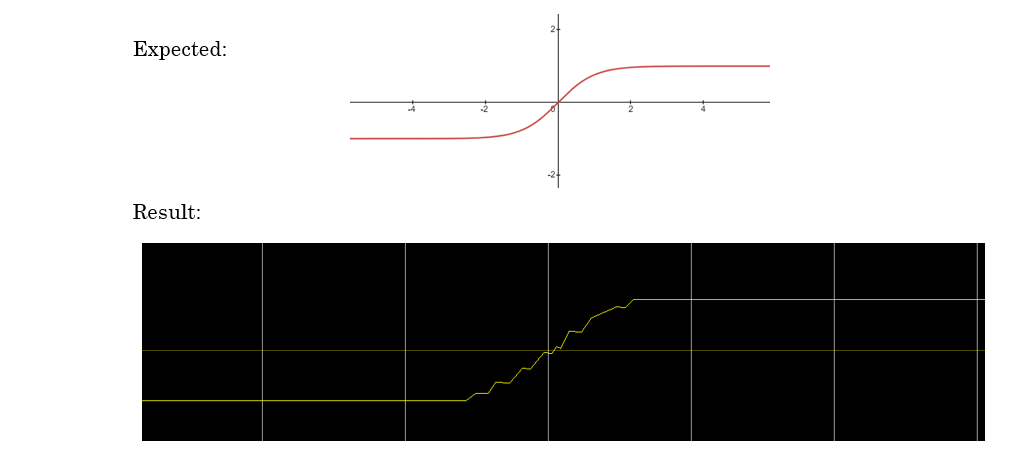
\includegraphics[width=0.8\textwidth]{tanh_expected_vs_simulation.png}
        \caption{Expected Vs Post Implementation Waveform of Tanh Fucntion}
        \label{fig:enter-label}
    \end{figure}
\begin{itemize}
    \item Here coarse nature of the tanh(z) waveform for z lying in the range of [-1,1] is attributed to the fact that inputs given to the module via testbench are not spaced very close to each other. Hence the obtained waveform is not as smooth as the expected waveform.
\end{itemize}

\section{Design Strategies Employed}
\begin{itemize}
    \item In the generation of the various trigonometric functions, 10 iterations are run in a combinational always block (\textit{always@(*)}) and the final result that we obtain after 10 iterations are updated in a register in a clocked always block(\textit{always@(poseedge clk)}). Asynchornous Reset has been employed in all the designs. 

    \item For the generation of sin(z), cos(z) and tan(z) functions, final result after 10 iterations was updated by a slower clock signal of frequency 3.33MHz as these values had to be sent to the PMOD DA2 DAC. This 3.33 MHz is arbitrary and any value less than 30MHz would do. The final result after  of  $tan^-1(y)$ and $tanh(z)$ are updated using 30ns clock and that of $tanh^{-1}(y)$ function is updated using 32ns clock. These specifications satisfy all the timing constraints. 
\end{itemize}

\section{Implementation Challenges}
\begin{itemize}
    \item For the implementation of sin(z) and cos(z), a slower clock signal \textit{clk2} was used as enable signal inside clocked always block of the original 100MHz clock signal (\textit{always@(posedge clk)}). Because of this, timing constraints were met only when $T_{clk}$ was set to 23ns. But when clk2 signal was not used just as an enable and when the final result was updated inside clocked always block of clk2 (\textit{always@(posedge clk2)}), timing constraints were met for $T_{clk}$ of 10ns with a positive slack.

    \item Since clk2 was generated using counters and the original clk of 100MHz, we used an asynchronous reset to support all the reset activities. This is because, when \textit{rst} signal was active, the counter used to generate clk2 signal was also reset and there were no more edges in clk2 signal. Hence asynchronous reset has been employed in all the designs

    \item For the functions $tanh(z)$ , $tan^{-1}(y)$, $tanh^{-1}(y)$, the inputs had to be given manually in the test bench and each design had its own fixed point representation (i.e, different number of bits before and after the binary point). Giving inputs manually was an arduous task. Hence a python script was programmed to generate input test vectors with the necessary precision. This accelerated the testing process. 
\end{itemize}

\section{Results}
\begin{itemize}
    \item The functions sin(z), cos(z), tan(z) were visualized on the oscilloscope.
    \item The functions tanh(z), $tan^{-1}(y)$, $tanh^{-1}(y)$, were verified through simulations in Xilinx Vivado.
    \item Timing Analysis was carried out for all the designs. Power reports are included in the final submission and not added in the report to maintain brevity of the report.
\end{itemize}

\section{Conclusions and Possible Improvements}
\begin{itemize}
    \item It was found that for functions that are bounded, CORDIC gave very good results. 
    \item For functions that are unbounded, CORDIC gave good results up to a certain point beyond which it was not possible to capture the results accurately due to fixed number of iterations and fixed point representation in the algorithm. 
    \item For functions involving division, results were good as long as the expected value lies in the range of [-2,2]. Beyond this range, the values saturate at 2. This was the case in tan(z) function. Fortunately, this was not fatal for the implementation of tanh(z) function because tanh(z) function takes values only within [-1,1].
    \item 10 iterations were used in this project for the generation of the various types of trigonometric functions. Number of iterations is the designer's choice. When more iterations are used, it is worthwhile to use \textit{pipeline} the design for faster results. Due to time constraints, the designs in this project are un-pipelined. 
    \item To conclude, when we want to implement whose results are bounded and do not need division CORDIC is a hardware friendly option. Because not a single * operator was used in the implementation of all the designs. However, when functions increase rapidly or if division computations are involved, one has to look for alternate options if accuracy is of high priority as CORDIC fails to provide good accuracy in these cases. 
\end{itemize}

 \section{Acknowledgements}
 \begin{itemize}
     \item Thanks to the instructor of the course Professor Debayan Das, for his guidance over the course of the mini project. 

     \item Thanks to ESE seniors Varsha, Swapnankit, Arimardan, Sachin Thomas, Vibhore Jain and classmate Elizabeth Kuruvilla for their inputs. 
     
 \end{itemize}
 
\section{References}
 \begin{itemize}
    \item Article on CORDIC in "allaboutcircuits.com" : https://www.allaboutcircuits.com/technical-articles/an-introduction-to-the-cordic-algorithm/

    \item NPTEL video:"  CORDIC Algorithm " by Prof Nitin Chandrachoodan , IITM. Lecture Series : \textit{Mapping Signal Processing Algorithms to Architecture}.
    \item NPTEL video:  " CORDIC Architecture " Prof. Indranil Hatai  . Lecture Series: \textit{Architectural Design of Digital integrated circuits}.
 \end{itemize}
\end{document}
